\documentclass[12pt]{article}
\usepackage[letterpaper,margin=1in]{geometry}
\usepackage[T1]{fontenc}
\usepackage{amsmath}
\usepackage{mathptmx}
\renewcommand{\ttdefault}{lmtt}
\usepackage{microtype}
\usepackage{setspace}\onehalfspacing
\usepackage{booktabs,threeparttable,tabularx,array,multirow,makecell}
\usepackage{graphicx,caption,enumitem,float}
\usepackage[authoryear,round]{natbib}
\usepackage{xcolor}
\usepackage[pdftitle={Do J.Crew Blockers Block? A Backtest of 91 Credit Agreements Against Eleven Real Dropdowns},pdfauthor={Saurav Sharma},pdfkeywords={liability management, J.Crew blocker, dropdown, leveraged loans, covenants},colorlinks=true,linkcolor=black,citecolor=blue!50!black,urlcolor=blue!50!black]{hyperref}
\usepackage{titlesec}
\titleformat{\section}{\large\bfseries}{\thesection.}{0.6em}{}
\titleformat{\subsection}{\normalsize\bfseries}{\thesubsection}{0.6em}{}
\captionsetup{font=small,labelfont=bf,labelsep=period,justification=centering}
\captionsetup[table]{skip=4pt}
\setlist{itemsep=2pt,topsep=4pt}
\newcolumntype{L}{>{\raggedright\arraybackslash}X}
\renewcommand{\arraystretch}{1.15}
\makeatletter\setlength{\@fptop}{0pt}\setlength{\@fpsep}{12pt}\setlength{\@fpbot}{0pt plus 1fil}\makeatother
\renewcommand{\topfraction}{0.85}\renewcommand{\textfraction}{0.1}\renewcommand{\floatpagefraction}{0.75}
\newcommand{\tabnote}[1]{\par\vspace{3pt}\begin{minipage}{\linewidth}\footnotesize\setstretch{1}\textit{Notes:} #1\end{minipage}}

\begin{document}
\begin{titlepage}\renewcommand{\thefootnote}{\fnsymbol{footnote}}
\centering\setstretch{1.2}
{\LARGE\bfseries Do J.Crew Blockers Block?\par}
\vspace{4pt}
{\Large A Backtest of 91 Credit Agreements Against Eleven Real Dropdowns\par}
\vspace{18pt}
{\large Saurav Sharma\thanks{Independent researcher. Email: \href{mailto:sauravsharma0369@gmail.com}{sauravsharma0369@gmail.com}. Data, code and pre-registrations: \url{https://github.com/saurav0369/jcrew-blockers}. I used language-model tools (Claude, Anthropic) for document search, first-pass coding and editing; every coding call the results rely on was checked by hand against the filing. All errors are mine.}\par}
\vspace{8pt}
{\normalsize November 2026\par}
\vspace{24pt}
\begin{minipage}{0.88\textwidth}\setstretch{1.15}\small
\centerline{\bfseries Abstract}\vspace{4pt}
Lenders now ask for ``J.Crew blockers'' in about half of new leveraged loans, but whether these clauses would stop the dropdowns borrowers actually execute has not, as far as I can find, been tested in public. I backtest 91 blockers, drawn at random from credit agreements filed with the SEC in 2020--2026, against eleven dropdowns completed without lender consent in 2016--2026. Scored clause by clause, the median blocker stops 2 of 11: J.Crew and Travelport, the two cases in which intellectual property alone went to an unrestricted subsidiary. Scored across the whole agreement, crediting the Pluralsight, Envision, Chewy and catch-all blockers found anywhere in the contract, the median is still 2 (3 if weak guarantee-release provisions count); 58 of 91 agreements stop at most three, 4 stop all eleven, and 52 stop none of the nine dropdowns that did not follow the J.Crew pattern. The result survives stricter and looser scoring rules, dropping any single event, and resampling the agreements. The misses trace to drafting choices: 87\% of blockers protect IP only, 87\% do not reach entities outside the group, 69\% do not reach non-guarantor subsidiaries, and only 4 of 91 are sacred rights, while 53 of the same contracts entrench protection against subordination. The agreement-level rule and its predictions were fingerprinted before the scan, two earlier prediction tests failed and are reported, and one script reproduces every number.

\vspace{8pt}
\noindent\textbf{JEL classification:} G23, G32, G33, K12, K22\\
\textbf{Keywords:} liability management, J.Crew blocker, dropdown, leveraged loans, covenants, sacred rights, backtest
\end{minipage}
\end{titlepage}\setcounter{footnote}{0}

\section{Introduction}
In a dropdown, a stressed borrower moves valuable assets out of its lenders' collateral and borrows against them elsewhere. After J.Crew moved its trademarks to an unrestricted subsidiary in 2016, lenders began asking for ``J.Crew blockers'': clauses barring the transfer of material intellectual property to unrestricted subsidiaries. Borrowers have since moved equity stakes (Bausch + Lomb, Chewy), business lines (MyTheresa, AmSurg), joint-venture interests (Trinseo) and whole asset bases (Del Monte), and have sent IP to subsidiaries that never guaranteed the loans (Revlon, Pluralsight) or to joint ventures outside the group (Xerox).

Blockers have spread fast. Noetica, which tracks deal terms, reports J.Crew protections in half of the deals it covered in Q2 2026, up from 15\% in Q1 2023, and Pluralsight blockers in 20\% \citep{Noetica2026}. Law firms and data vendors describe and grade how blockers are drafted \citep{Cleary2025,Octus2025}. What has not been published, as far as my searches reached, is a test of whether the clauses would have stopped the transactions they exist to prevent.

I run that test as a backtest. Each realized dropdown is an attack, each agreement's protections are the defence, and every pair is scored against the contract text under one mechanical rule. I score twice: the J.Crew clause alone (Section~\ref{sec:clause}), and then the whole agreement, crediting every named blocker anywhere in the contract (Section~\ref{sec:stack}), under a rule fixed and fingerprinted before the scan. The answer is the same both ways: \emph{the median agreement stops 2 of 11 real dropdowns}, and more than half of agreements stop none of the nine dropdowns that did not follow the original J.Crew pattern.

The paper makes five contributions:
\begin{enumerate}
\item a random-sample census of 91 blockers in SEC-filed credit agreements, each coded on six dimensions with a verbatim quote and a link to the filing;
\item an attack library of eleven non-consensual dropdowns (2016--2026), each traced to an opened source and independently fact-checked;
\item a backtest at clause level and at whole-agreement level, the latter pre-registered, both reproducible from the released data with one script;
\item evidence that the gaps persist in contracts filed in 2025--2026, and that blockers are rarely sacred rights while anti-subordination protection usually is;
\item three earlier tests of whether contract terms predict dropdowns, two of which failed, reported in full.
\end{enumerate}

\paragraph{Related literature.} The closest academic work is \citet{BuccolaNini2024}, who code loan contracts around J.Crew (2016) and Serta (2020) and find that loans originated after Serta became much more likely to block uptiers, while susceptibility to dropdowns changed little after J.Crew. The sacred-rights contrast in Section~\ref{sec:gaps} is a later-sample observation, on a different measure, consistent with their result. \citet{IvashinaVallee2025} map carve-outs in 1,240 leveraged loan agreements and show how baskets and exceptions weaken negative covenants; I study one protection in depth and test it against outcomes rather than measuring its prevalence or price. Practitioner work catalogues the named blockers and where they sit in an agreement, and notes that effective protection may need several of them \citep{Cleary2025}. \citet{Octus2025} grades European J.Crew blockers from their drafting, without testing them against past transactions, and \citet{Noetica2026} tracks prevalence. I found no public, systematic backtest of blocker text against realized dropdowns; paid databases were not searched.

\section{Data}\label{sec:data}
\paragraph{Sampling frame.} An EDGAR full-text search for ``Material Intellectual Property'', ``Unrestricted Subsidiary'' and ``Credit Agreement'' in EX-10 exhibits filed 1 January 2020 to 19 November 2026, keeping the first filing per company, returned 504 companies. Two seeded random draws (seeds 20261120 and 20261121) produced 102 agreements carrying a blocker, of which 91 had blocker text readable for coding.

\paragraph{Coding.} Each agreement was coded on the six dimensions in Table~\ref{tab:coding}. Two independent first-pass coders split the agreements, blind to earlier labels, and gave a verbatim quote for every answer; every call was then checked against the filing. Table~\ref{tab:verify} reports the checks; the released data mark every corrected row.

\begin{table}[!htbp]\centering
\begin{threeparttable}
\caption{Coding dimensions}\label{tab:coding}
\begin{tabularx}{0.85\linewidth}{Ll}
\toprule
Dimension & Values\\\midrule
Reaches non-guarantor restricted subsidiaries & Yes / No\\
Reaches entities outside the group (JVs, sister companies) & Yes / No\\
Assets protected & IP only / IP and other assets\\
Who decides materiality & Borrower / agent / not named / undefined\\
Covers exclusive licences & Yes / No\\
Blocker is a sacred right & Yes / No\\
\bottomrule
\end{tabularx}
\end{threeparttable}
\end{table}

\begin{table}[!htbp]\centering
\begin{threeparttable}
\caption{Verification of the coding}\label{tab:verify}
\begin{tabularx}{0.92\linewidth}{Ll}
\toprule
Check & Result\\\midrule
Independent second reader on blocker tiers (29 random agreements) & 27 agree; Cohen's $\kappa=0.84$\\
Hand check of scope coding (15 random) & 13 agree; both misses corrected\\
Hand check of materiality coding (14) & 13 agree; 3 corrections in total\\
Independent fact-check of dropdowns & 12 of 14 agree; 1 excluded\\
Sacred rights & 4 matches read in full; 39 others incidental\\
\bottomrule
\end{tabularx}
\end{threeparttable}
\end{table}

\section{The attack library}\label{sec:attacks}
Eleven dropdowns enter the test and three more are shown but excluded (Appendix Table~\ref{tab:events}). Each row was built from primary sources and re-checked independently by a second reader who did not see the first's work. Consent transactions (AMC, STG) are excluded because a blocker that lenders themselves vote away was not circumvented; Revlon BrandCo is excluded because its destination could not be confirmed. The list is the set of dropdowns that public reporting documents, not a random sample.

\section{Backtest results}\label{sec:results}
\subsection{The J.Crew clause}\label{sec:clause}
Each dropdown $e$ is described by the assets it moved, $a_e\in\{\text{IP},\text{non-IP}\}$, and its route over three destination types: unrestricted subsidiaries ($U$), non-guarantor restricted subsidiaries ($R$) and entities outside the group ($N$). A route is either sequential ($d_1\to d_2$, any step can be blocked) or parallel ($d_1+d_2$, every destination must be blocked). Each blocker $b$ is described by the set of destinations it reaches, $D_b\ni U$, and whether its asset scope goes beyond IP, $x_b\in\{0,1\}$. Blocker $b$ covers destination $d$ for event $e$ if
\begin{equation}
c(b,d,e)=\mathbf{1}\{d\in D_b\}\cdot\mathbf{1}\{a_e=\text{IP}\ \lor\ x_b=1\},
\end{equation}
and stops the event if
\begin{equation}
s(b,e)=\begin{cases}\max_{d\in\text{route}(e)} c(b,d,e) & \text{sequential route},\\ \min_{d\in\text{route}(e)} c(b,d,e) & \text{parallel route}.\end{cases}
\end{equation}
A blocker's score is $\sum_{e}s(b,e)$ over the eleven events. The rule reads the clause as written: $R$ and $N$ enter $D_b$ only where the clause names them, and $x_b=1$ only where it names assets beyond IP.

The median blocker stops 2 of the 11 dropdowns: J.Crew and Travelport, the two cases in which IP alone went straight to an unrestricted subsidiary, which is the exact pattern the clause was written for (Figure~\ref{fig:stops}). The distribution is lopsided: 56 of 91 blockers stop only these two, and 3 of 91 stop all eleven. No blocker stops fewer than two, because every blocker in the sample at least bars IP moving to an unrestricted subsidiary.

Two cautions apply. First, the rule treats any mention of assets beyond IP as covering every asset, so the counts for non-IP moves are upper bounds. Second, ``stops'' means the clause, read as written, reaches the move; it does not mean a court would enforce it that way.

\begin{figure}[!t]\centering
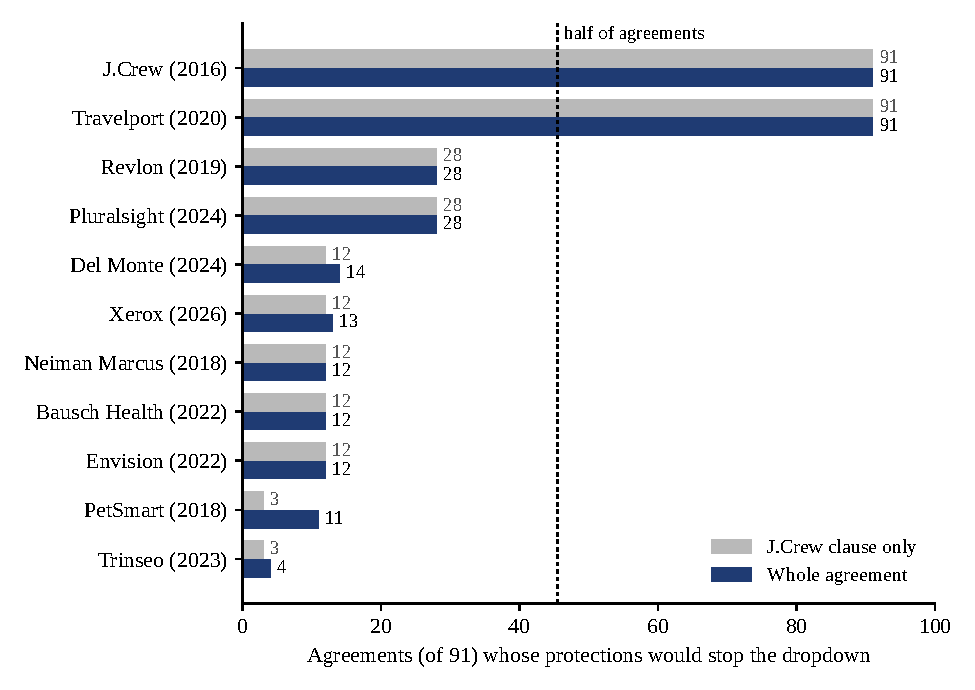
\includegraphics[width=0.95\linewidth]{fig1.pdf}
\caption{Agreements whose protections would stop each real dropdown}\label{fig:stops}
\begin{minipage}{0.92\linewidth}\footnotesize\setstretch{1}\textit{Notes:} Grey bars score the J.Crew clause alone (Section~\ref{sec:clause}); dark bars score the whole agreement (Section~\ref{sec:stack}). The dashed line marks half of the 91 agreements. Source: author's backtest; data and code in the replication package.\end{minipage}
\end{figure}

\subsection{Does the whole agreement block?}\label{sec:stack}
Market practice layers named blockers: Pluralsight provisions in the investment covenant, Envision provisions on designating unrestricted subsidiaries, Chewy provisions on guarantee release, and occasional catch-all ``omni'' blockers \citep{Cleary2025}. A J.Crew clause should not be blamed for missing a move another clause was written for, so I re-scored every agreement as a whole.

Before scanning, I fixed and fingerprinted the detection patterns, the stop rule and five predictions.\footnote{The pre-registration and its SHA-256 fingerprint are in the replication package. One clarification was logged before any score was computed: a Chewy provision counts against PetSmart only if a transfer to an affiliate cannot obtain the release through a borrower-judged purpose test or spare investment capacity (``strong'').} Keyword scans of all 91 agreements returned 248 passages, and every one was read. Pluralsight-type and outside-the-group protections added nothing: every hit was a J.Crew clause already coded. Chewy provisions appear in 21 of 91 agreements, 8 of them strong. One agreement, Cumulus, written after its own 2024 exchange, carries an omni-blocker; one other bars designating a subsidiary that holds substantially all assets.

At the agreement level the median contract still stops 2 of 11 (3 if weak Chewy provisions count); 58 of 91 stop at most three and 4 stop all eleven. Only PetSmart moves materially, from 3 agreements to 11 (24 counting weak provisions). Table~\ref{tab:prereg} shows that all five predictions held; Section~\ref{sec:robust} tests how much the result depends on the scoring rule.

\begin{table}[!htbp]\centering
\begin{threeparttable}
\caption{Pre-registered predictions for the whole-agreement backtest}\label{tab:prereg}
\begin{tabularx}{0.9\linewidth}{Lcc}
\toprule
Prediction & Observed & Result\\\midrule
Median agreement stops at most 3 of 11 & 2 & Held\\
At least half of agreements stop at most 3 & 64\% & Held\\
Chewy provisions in fewer than half of agreements & 23\% & Held\\
Omni-blockers in at most 3 agreements & 1 & Held\\
Pluralsight-type provisions add non-guarantor reach to under 15\% & 0\% & Held\\
\bottomrule
\end{tabularx}
\end{threeparttable}
\end{table}

Two biases pull in opposite directions. A keyword scan misses protections worded without the searched terms, which understates protection; combining provisions from different clauses credits coverage no single clause gives, which overstates it.

\subsection{Robustness}\label{sec:robust}
Table~\ref{tab:robust} rescores the backtest under alternative rules. Denying all credit for non-IP coverage leaves the median at 2. Counting weak Chewy provisions raises it to 3. Dropping any one of the eleven events leaves the whole-agreement median at 1 or 2. Resampling the 91 agreements 10,000 times gives a 95\% interval of [2, 3] for the median and 54--74\% for the share of agreements that stop at most three dropdowns.

The sharpest form of the result removes J.Crew and Travelport, the two cases the clause was written for. Against the remaining nine dropdowns, 52 of 91 agreements (57\%; 95\% interval 47--67\%) stop none at all, even scored as whole agreements.

\begin{table}[!t]\centering
\begin{threeparttable}
\caption{Robustness of the headline result}\label{tab:robust}
\begin{tabularx}{0.95\linewidth}{Lccc}
\toprule
Scoring rule & \makecell{Median\\stopped} & \makecell{Stop at\\most 3} & \makecell{Stop\\all 11}\\\midrule
Clause level (baseline) & 2 & 58 & 3\\
Clause level, no credit for non-IP coverage & 2 & 63 & 0\\
Whole agreement, strong Chewy (baseline) & 2 & 58 & 4\\
Whole agreement, weak Chewy also counts & 3 & 58 & 4\\
Whole agreement, dropping any one event & 1--2 & 58--69 & ---\\
Whole agreement, bootstrap 95\% interval & [2, 3] & 54--74\% & ---\\\midrule
Whole agreement, nine non-J.Crew-pattern events only & 0 & \multicolumn{2}{c}{52 of 91 stop none}\\
\bottomrule
\end{tabularx}
\tabnote{Counts are of the 91 agreements. The bootstrap resamples agreements with replacement (10,000 draws, seed 20261123). Computed in the replication package.}
\end{threeparttable}
\end{table}

\section{Six gaps}\label{sec:gaps}
The misses trace to six recurring drafting choices (Table~\ref{tab:gaps}). Each is a field in the released data, and each row links to the clause on EDGAR. Table~\ref{tab:clauses} shows what the difference looks like in the contract text: a typical blocker, which stops 2 of the 11 dropdowns, beside two that stop all eleven.

\begin{table}[!t]\centering
\begin{threeparttable}
\caption{What a narrow and a broad blocker say}\label{tab:clauses}
\small\setstretch{1}
\begin{tabularx}{\linewidth}{>{\raggedright\arraybackslash}p{0.17\linewidth}Lc}
\toprule
Agreement & Operative text (excerpt) & Stops\\\midrule
Hovnanian (2024) & ``no Restricted Subsidiary may transfer \ldots{} sell or otherwise dispose of, or grant an exclusive license in, any Material Intellectual Property to an Unrestricted Subsidiary and \ldots{} no Unrestricted Subsidiary may, at any time, own, or hold an exclusive license in, any Material Intellectual Property'' & 2 of 11\\\addlinespace
Sealed Air (2025) & ``neither the Company nor any of its Restricted Subsidiaries shall consummate any transaction that results \ldots{} in the transfer (including an exclusive license) of any Material Intellectual Property or Material Manufacturing Facility \ldots{} to (x) any Restricted Subsidiary that is not a Loan Party \ldots{} or (y) any Affiliate that is not the Company or a Restricted Subsidiary unless \ldots{} such transfer is made on an arm's length basis'' & 11 of 11\\\addlinespace
Cumulus (2024) & ``in no event shall any Issuer or any other Guarantor sell, transfer or otherwise dispose of any Material Intellectual Property or any other assets \ldots{} that is material to the business \ldots{} to any Subsidiary that is not an Issuer or a Guarantor''; the Unrestricted Subsidiary concept is removed and its re-introduction made a sacred right & 11 of 11\\
\bottomrule
\end{tabularx}
\tabnote{Excerpts are quoted from the coded exhibits (for Cumulus, the 2024 exchange documents filed with the SEC); ellipses mark omitted text. ``Stops'' is the whole-agreement score. Sealed Air's clause reaches non-guarantor subsidiaries and affiliates outside the group and covers a named class of non-IP assets; Hovnanian's reaches only unrestricted subsidiaries and only IP.}
\end{threeparttable}
\end{table}

\begin{table}[!htbp]\centering
\begin{threeparttable}
\caption{Six drafting gaps in 91 J.Crew blockers}\label{tab:gaps}
\begin{tabularx}{\linewidth}{Llcl}
\toprule
Gap & Blockers & 95\% CI & Dropdowns it lets through\\\midrule
Not a sacred right & 87/91 (96\%) & 89--98 & AMC, STG (by consent)\\
Protects IP only & 79/91 (87\%) & 78--92 & Neiman, PetSmart, Bausch,\\
 & & & Envision, Del Monte, Trinseo\\
Does not reach outside the group & 79/91 (87\%) & 78--92 & Xerox, Trinseo\\
Does not reach non-guarantor subs & 63/91 (69\%) & 59--78 & Revlon, Pluralsight\\
Silent on exclusive licences & 41/89 (46\%) & 36--56 & Licence-based moves\\
Borrower decides ``material'' & 26/72 (36\%) & 26--48 & Moves deemed immaterial\\
\bottomrule
\end{tabularx}
\tabnote{Intervals are Wilson 95\% intervals. A blocker that is not a sacred right can be removed by Required Lenders (a simple majority). Exclusive-licence coverage is a share of the 89 blockers that could be coded; borrower-decided materiality is a share of the 72 blockers whose definition sets a materiality test.}
\end{threeparttable}
\end{table}

\subsection{Sacred rights: 4 of 91}
Only four blockers are entrenched as sacred rights, amendable only with each affected lender's consent: Gannett, Cumulus, Vacasa and Cano Health. For the other 87, an unentrenched blocker still forces the borrower to win a majority vote, but a majority that is offered a better deal can remove it, which is what happened at AMC and STG in 2024. I pre-registered that fewer than 25\% would be entrenched; the result (4\%) held. The count is a floor: each agreement was scanned three ways (a window around every unanimity phrase, a search for the blocker's own section number near consent language, and a sweep for ``have the effect of'' and unrestricted-subsidiary wording), and every match was read, but a protection that names neither the blocker nor its section would be missed.

\subsection{The contrast: anti-subordination is usually entrenched}
By comparison, 53 of 91 contracts (58\%) make lien or payment subordination a sacred right, the protection added after uptier exchanges such as Serta. I extracted every passage within about 500 characters of both ``subordinat'' and an each-lender consent phrase (55 contracts had one), read them all, and excluded two. This is an observation, not a pre-registered test, and it does not separate lien-only from payment protection. Read with the previous subsection, it suggests that lenders entrenched protection against uptiers far more often than against dropdowns, consistent with \citet{BuccolaNini2024}.

\section{Over time}\label{sec:time}
If lenders learned from each new dropdown, later blockers should reach further. Table~\ref{tab:vintage} groups the 91 by the year their agreement was filed. The median blocker stops two of the eleven dropdowns in every period. Coverage of exclusive licences roughly doubled and asset scope widened a little, but reach to non-guarantor subsidiaries and outside the group did not improve, and the share of blockers that let the borrower decide what is ``material'' rose from 15\% to 40\%. All four entrenched blockers were filed in 2024; none of the 30 filed in 2025--2026 is entrenched.

\begin{table}[!htbp]\centering
\begin{threeparttable}
\caption{Blocker coverage by filing year}\label{tab:vintage}
\small
\begin{tabular}{lcccccccc}
\toprule
Filed & $N$ & \makecell{Median\\stopped} & \makecell{Non-guar.\\subs} & \makecell{Outside\\group} & \makecell{Beyond\\IP} & \makecell{Borrower\\decides} & \makecell{Excl.\\licences} & \makecell{Sacred\\right}\\\midrule
2020--2022 & 41 & 2 & 34\% & 20\% & 7\% & 15\% & 34\% & 0\\
2023--2024 & 20 & 2 & 25\% & 0\% & 20\% & 40\% & 65\% & 4\\
2025--2026 & 30 & 2 & 30\% & 13\% & 17\% & 40\% & 70\% & 0\\
\bottomrule
\end{tabular}
\tabnote{Groups are small and coded from the earliest filed exhibit, so later amendments are not reflected. The table describes drift; it is not a test.}
\end{threeparttable}
\end{table}

\section{Prediction tests}\label{sec:prediction}
Before the backtest, this project tried to predict dropdowns from contract text. Table~\ref{tab:predict} reports those tests in full because two of three did not work.

\begin{table}[!htbp]\centering
\begin{threeparttable}
\caption{Earlier tests of whether contract terms predict dropdowns}\label{tab:predict}
\small
\begin{tabularx}{\linewidth}{>{\raggedright\arraybackslash}p{0.27\linewidth}>{\raggedright\arraybackslash}p{0.2\linewidth}L}
\toprule
Test & Pre-registered bar & Result\\\midrule
Blind retrodiction: predict the route from the pre-event agreement & At least 2 of 3 cases match & Passed formally, 2 of 3. Trinseo informative (route found in a 2017 agreement, used in 2023); Bausch uninformative (route named in 2022); AMC failed (a consent transaction).\\
Exit capacity as a share of assets, events vs.\ controls & Controls outside the event range & No usable separation. Events 1.7--11.2\%; controls 0.0--7.7\%.\\
``Soft unlimited exit'' rule, 4 new events and 6 controls & $\geq$3 of 4 events, $\leq$2 of 6 controls & Failed: 2 of 4 events flagged.\\
\bottomrule
\end{tabularx}
\end{threeparttable}
\end{table}

One pattern emerged after the controls were seen. In both informative event cases, the unlimited route sat behind a test a stressed company could pass: Trinseo's fixed-charge ratio needed only to be no lower than before, and Bausch's remaining-company leverage cap was 7.60x. The controls' unlimited routes sat behind tests a stressed company is unlikely to pass. This is a hypothesis for new cases, not a finding. What survived is the narrower, checkable claim of Sections~\ref{sec:results}--\ref{sec:gaps}: what the clauses say, and which documented moves they reach.

\section{Discussion}\label{sec:discussion}
\paragraph{A blocker is a patch for one exploit.} The typical clause bars material IP from moving to an unrestricted subsidiary. It reliably stops J.Crew and Travelport. It does not reach the routes later borrowers took: non-IP value (Neiman, PetSmart, Bausch), non-guarantor restricted subsidiaries (Revlon, Pluralsight), or entities outside the group (Trinseo, Xerox), and the rest of the agreement rarely fills the gap: 52 of 91 agreements stop none of the nine later-pattern dropdowns. A lender who reads ``J.Crew blocker'' on a term sheet as general protection against dropdowns is buying less than the label suggests.

\paragraph{What is entrenched differs from what is attacked.} In 2024, AMC and STG showed that a blocker which is not a sacred right can be removed by a majority that is offered a better deal. Only 4 of 91 blockers are entrenched against that, while 53 of the same agreements entrench protection against subordination.

\paragraph{Newer documents have not closed the gap.} Licence coverage improved. Reach to non-guarantor subsidiaries and outside the group did not, and borrower-determined materiality became more common.

\paragraph{For drafters,} the six gaps map to six edits: cover all material assets, not only IP; reach non-guarantor restricted subsidiaries and non-subsidiary affiliates; name exclusive licences; use an objective materiality test; and make the blocker a sacred right. Whether any of these would survive negotiation or hold up in court is outside this paper's evidence.

\section{Limits, pre-registration and disclosure}\label{sec:limits}
\paragraph{Limits.}
\begin{itemize}
\item \emph{The 14 dropdowns are not a random sample.} They are the cases public reporting documents.
\item \emph{No lawyer has reviewed the coding.} First-pass coding used language-model tools and every call was checked by hand. A 20-contract stratified audit sheet (seed 20261123) is prepared for practitioner review, and its results will be reported whatever they show.
\item \emph{Later amendments are not reflected.} Coders read the earliest filed credit-agreement exhibit.
\item \emph{The stop rule is mechanical.} It reads clauses as written and ignores other debt documents, intercreditor terms and litigation risk.
\item \emph{The sacred-rights count is a floor,} and the subordination count ties consent level to clauses by proximity and was not pre-registered.
\item \emph{The agreement-level scan is keyword-based.} It reads every passage it flags but cannot see a protection worded without the searched terms.
\item \emph{The sample is public-company filers.} Most dropdowns happen at sponsor-backed private borrowers, whose documents may differ.
\end{itemize}

\paragraph{What was fixed in advance.} Each pre-registration was written and dated before the results it governs were seen. For four of them (the census thresholds, the whole-agreement rule, the retrodiction protocol and the soft-unlimited-exit rule) a SHA-256 recorded at the time of writing still matches the released file, and the replication package verifies it. They fixed the three census thresholds (all held on point estimates; the confidence intervals for outside-group reach and non-IP coverage extend to about 20\% and 22\%), the sacred-rights prediction, the retrodiction protocol, the soft-unlimited-exit rule, and the agreement-level rule with its five predictions. The clause-level stop rule was written after the scope coding came in.

\paragraph{Disclosure.} Document search, first-pass coding, fact-checking and editing used language-model tools (Claude, Anthropic). Every reading the results rely on was verified by hand against the filing. No outside person has reviewed this work.

\paragraph{Data and code availability.} All data, coding outputs, pre-registrations and code are at \url{https://github.com/saurav0369/jcrew-blockers}. Running \texttt{python3 reproduce.py} recomputes every number in this paper from the data files and exits with an error if any differs; planted faults were shown to make it fail.

\setstretch{1}
\bibliographystyle{apalike}
\bibliography{refs}
\nocite{JCrew2017,AMC2024,Bausch2022,Revlon2023,Trinseo2023}

\clearpage
\appendix
\section{The attack library}\label{app:events}
\begin{table}[H]\centering
\begin{threeparttable}
\caption{Dropdowns in the attack library}\label{tab:events}
\small\setstretch{1}
\begin{tabularx}{\linewidth}{clLLl}
\toprule
Year & Borrower & What moved & Where it went & In the test\\\midrule
2016 & J.Crew & Trademarks & Non-guarantor sub, then unrestricted sub & Yes\\
2018 & Neiman Marcus & MyTheresa business & Unrestricted sub, then parent & Yes\\
2018 & PetSmart & 36.5\% of Chewy equity & Unrestricted sub and sponsor & Yes\\
2019 & Revlon & American Crew trademarks & New non-guarantor subsidiary & Yes\\
2020 & Travelport & IP valued $\sim$\$1.15bn & Unrestricted subs & Yes\\
2022 & Bausch Health & Holder of 88.7\% of Bausch + Lomb & Unrestricted sub & Yes\\
2022 & Envision & AmSurg surgical-center entities & Unrestricted subs & Yes\\
2023 & Trinseo & 50\% Americas Styrenics JV stake & Sister company outside the group & Yes\\
2024 & Pluralsight & Intellectual property & Non-guarantor restricted sub & Yes\\
2024 & Del Monte & Substantially all assets & Intermediate sub, then unrestricted sub & Yes\\
2026 & Xerox & Core IP incl.\ trademarks & Joint venture outside the group & Yes\\\midrule
2024 & AMC & 175 theatres and the AMC brand & Unrestricted sub & No: consent\\
2024 & STG Logistics & Substantially all assets & Unrestricted subs & No: consent\\
2020 & Revlon BrandCo & BrandCo IP & Not confirmed & No: unverified\\
\bottomrule
\end{tabularx}
\tabnote{Sources: SEC filings and court opinions where available (J.Crew, Trinseo, AMC, Bausch Health, Revlon), otherwise law-firm commentary: King \& Spalding (Neiman Marcus), Cleary Gottlieb (PetSmart), Locke Lord (Travelport), Sidley (Envision), Goodwin (Pluralsight), Cadwalader (Del Monte), Winston \& Strawn (Xerox), Mayer Brown (STG). Full source links are in the replication package.}
\end{threeparttable}
\end{table}
\end{document}
